\pagestyle{aaron}
\section{Vergleich lineares/nichtlineares System} \label{sec:Vergleich}

In \autoref{fig:Bild4.1} ist die Übersicht der notwendigen Simulationsstruktur dargestellt. Aus der Übersicht geht hervor, dass beide Systeme unterschiedliche Eingänge besitzen und somit ein direkter Vergleich ohne entsprechende Berücksichtigung der Linearisierungsvorschriften unmöglich ist. Das linearisierte Modell verwendet als Eingang im Gegensatz zum nichtlinearen Modell eine Differenz $\Delta u$. Die Strukturen des nichtlinearen und des linearen Modells sind zur Information in \autoref{fig:Bild4.2} und \autoref{fig:Bild4.3} visualisiert.

\begin{figure}[H]
   \centering
   \fbox{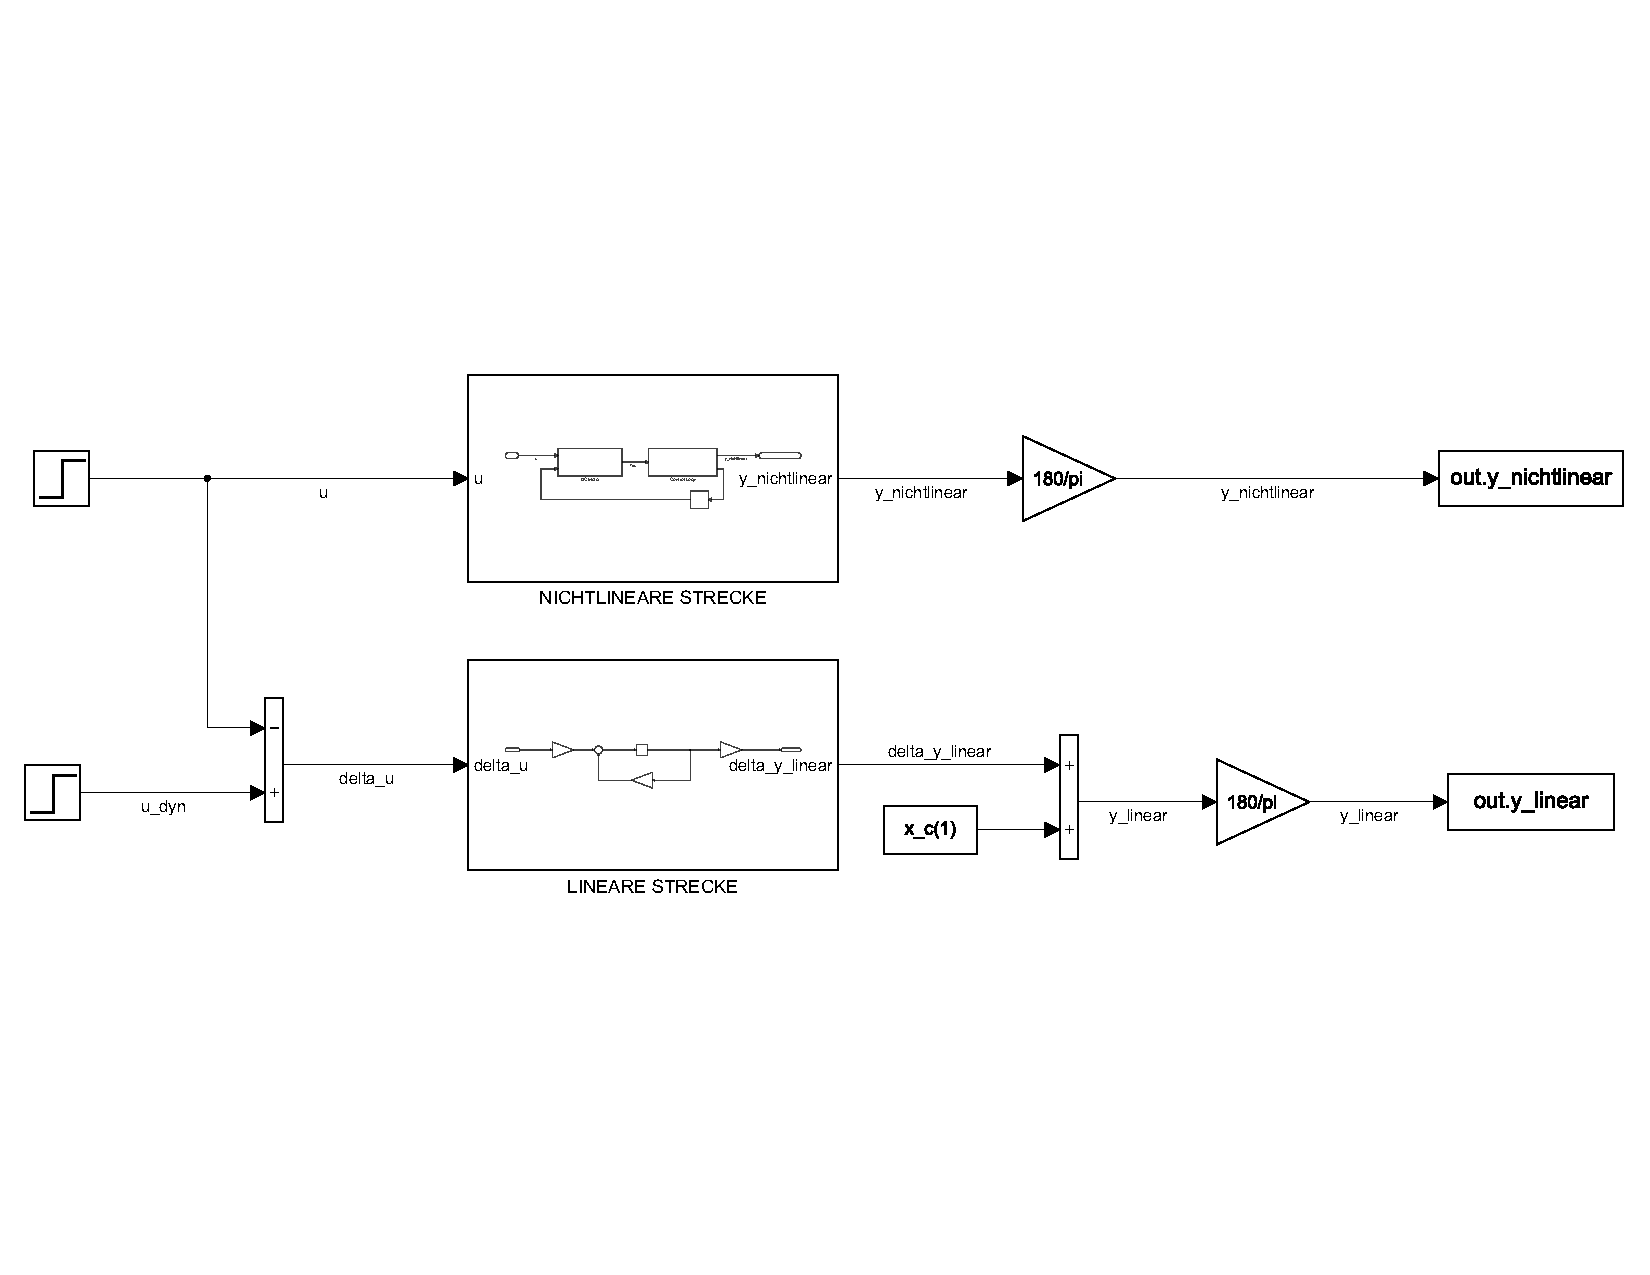
\includegraphics[width=0.65\textwidth]{Bilder/4. vergleich/system.pdf}}
   \caption[Übersicht der Simulationsstruktur]{Übersicht der Simulationsstruktur}
   \label{fig:Bild4.1}
\end{figure}

\begin{figure}[H]
   \centering
   \fbox{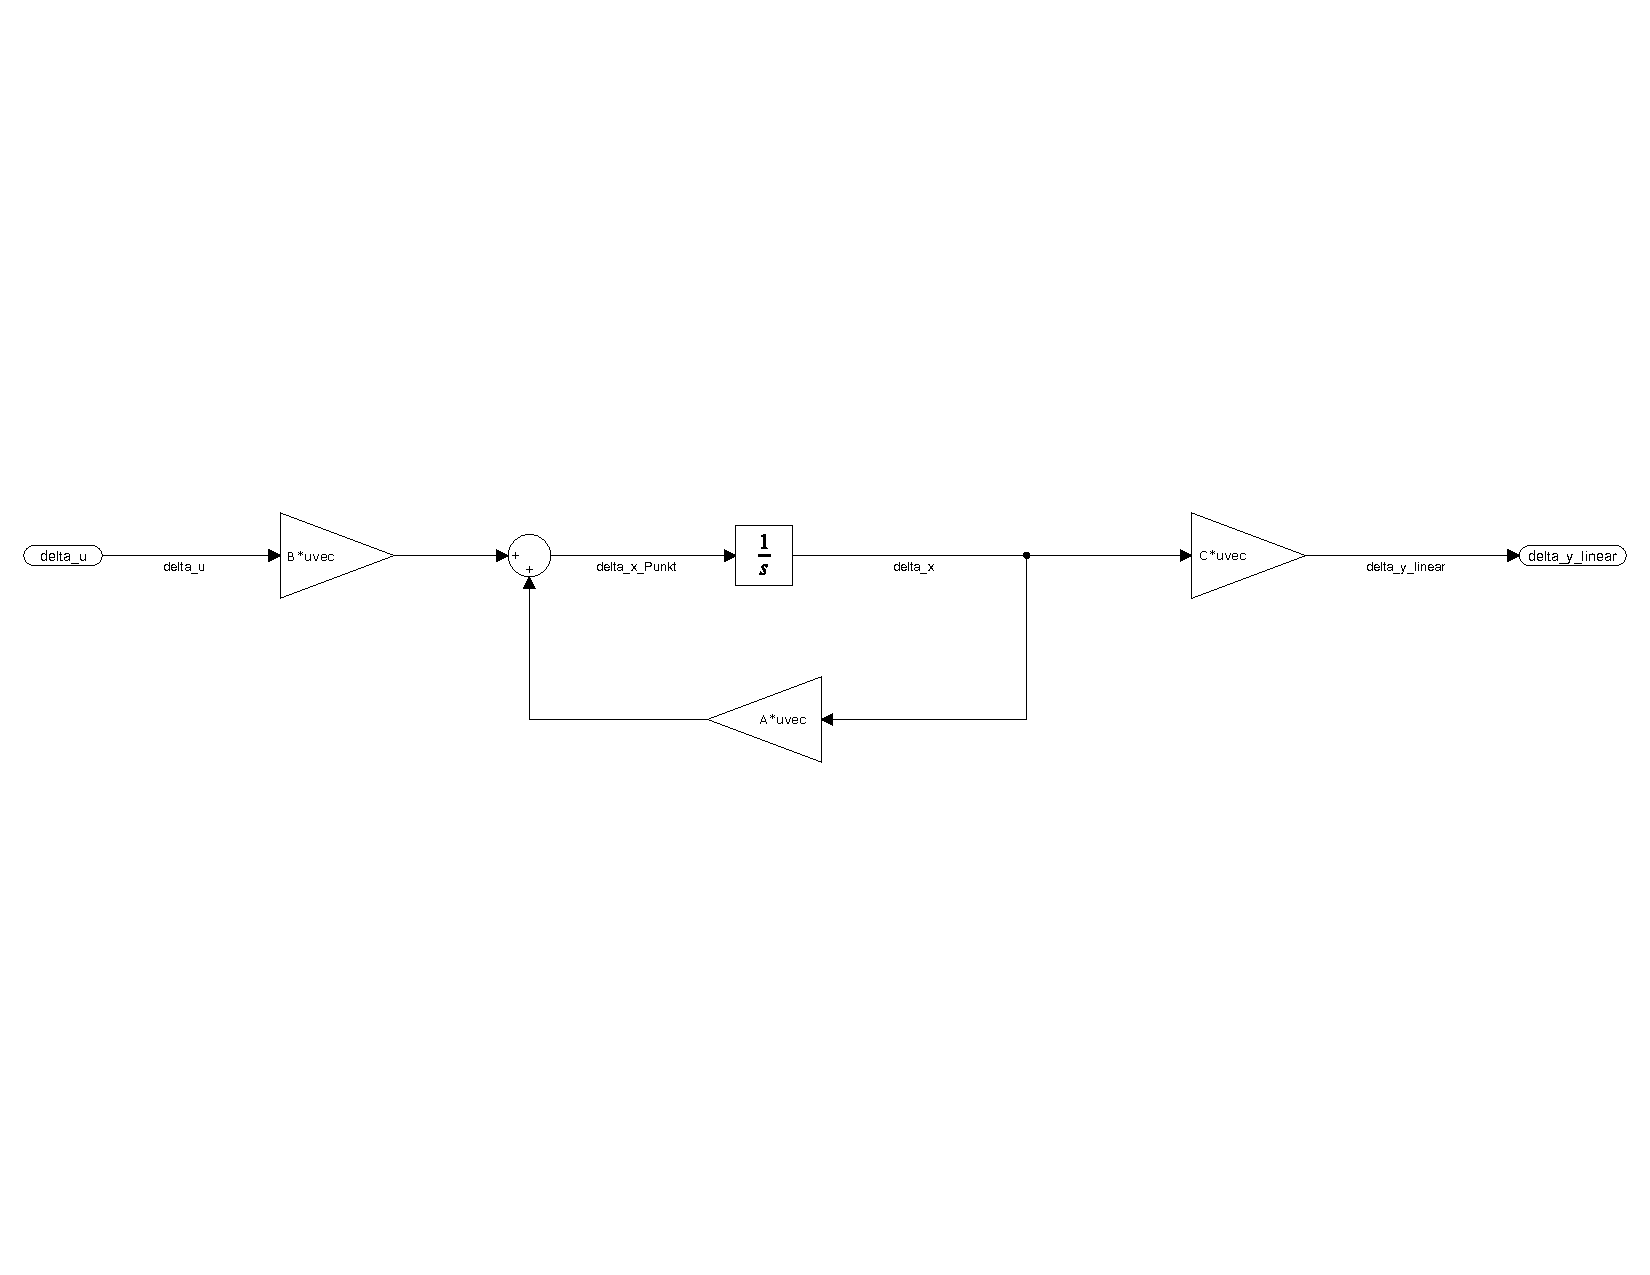
\includegraphics[width=0.65\textwidth]{Bilder/4. vergleich/linear.pdf}}
   \caption[Nichtlineare Strecke]{Nichtlineare Strecke}
   \label{fig:Bild4.2}
\end{figure}

\begin{figure}[H]
   \centering
   \fbox{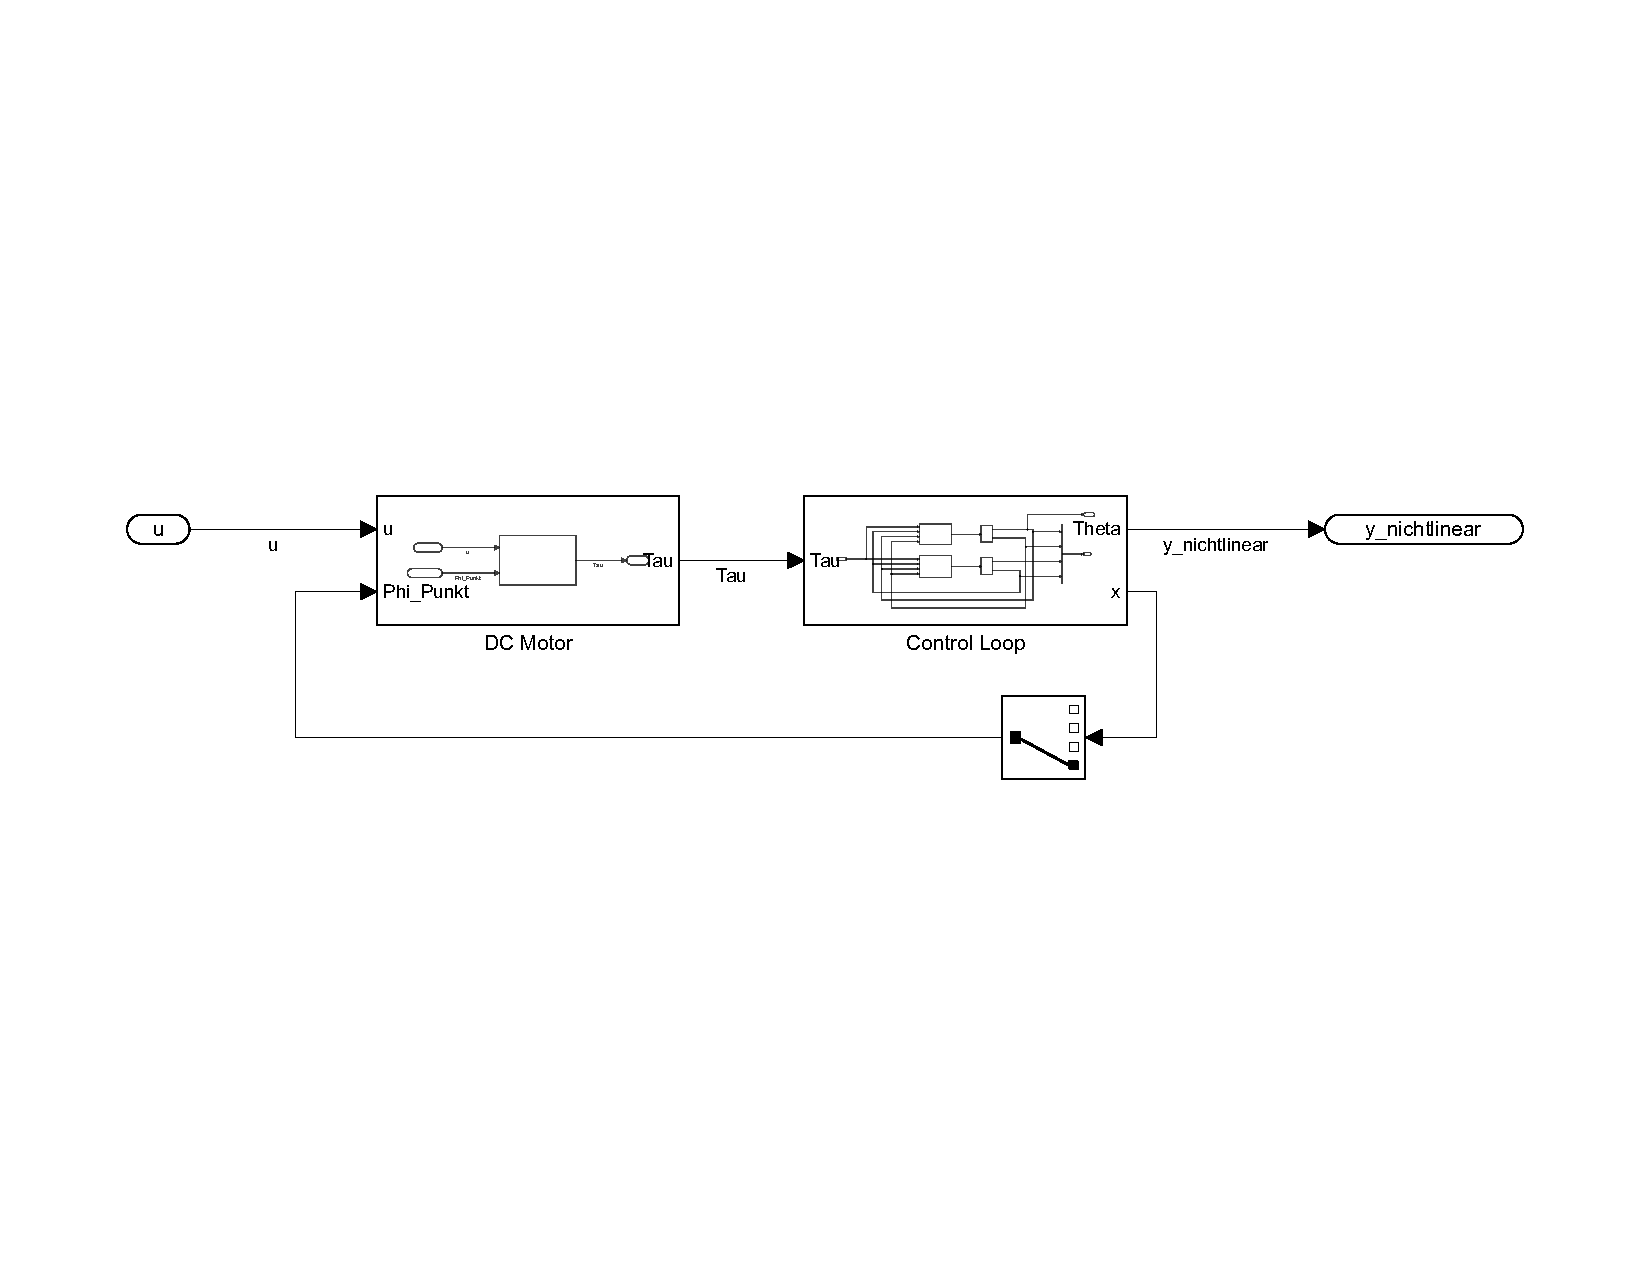
\includegraphics[width=0.65\textwidth]{Bilder/4. vergleich/nichtlinear.pdf}}
   \caption[Lineare Strecke]{Lineare Strecke}
   \label{fig:Bild4.3}
\end{figure}

Um das lineare mit dem nichtlinearen Modell zu vergleichen, werden gemäß \autoref{sec:Zustandsraumdarstellung} zu den Zuständen $\Delta \underline{x}$ die Ruhelagen $\underline{x}^*$ aus \autoref{eq:Gleichung3.10} addiert. Aus der \autoref{fig:Bild4.4} und \autoref{fig:Bild4.5} geht hervor, dass die implementierten Systeme für kleine Abweichungen von der Ruhelagen mit steigender Zeit $"t"$ selbiges Verhalten aufweisen.

\begin{figure}[H]
   \centering
   \fbox{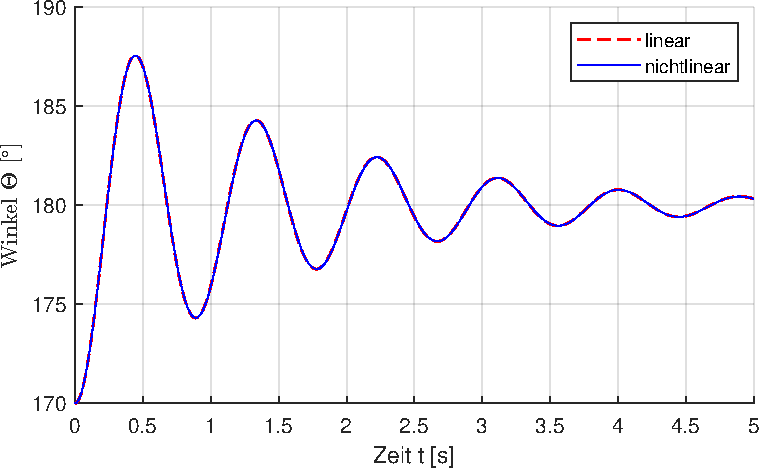
\includegraphics[width=0.7\textwidth]{Bilder/4. vergleich/vergleich_10_grad.pdf}}
   \caption[Vergleich der Pendelwinkel $\theta$ - kleine Auslenkung]{Vergleich der Pendelwinkel $\theta$ bei -10${^\circ}$ Anfangsauslenkung zur Ruhelage}
   \label{fig:Bild4.4}
\end{figure}

\begin{figure}[H]
   \centering
   \fbox{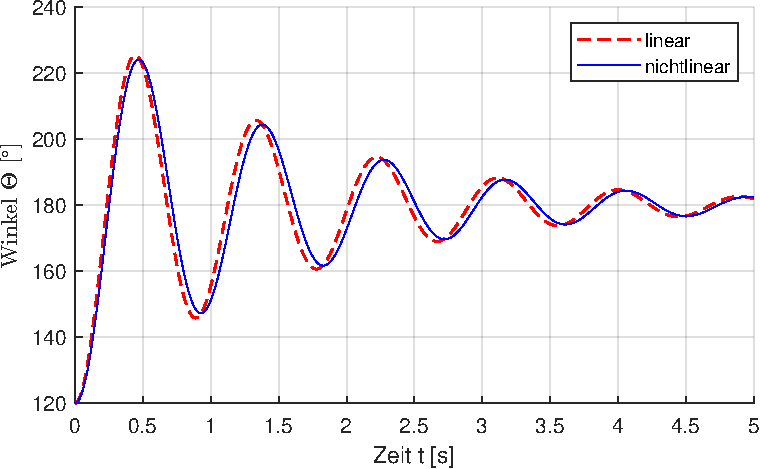
\includegraphics[width=0.7\textwidth]{Bilder/4. vergleich/vergleich_60_grad.pdf}}
   \caption[Vergleich der Pendelwinkel $\theta$ - große Auslenkung]{Vergleich der Pendelwinkel $\theta$ bei -60${^\circ}$ Anfangsauslenkung zur Ruhelage}
   \label{fig:Bild4.5}
\end{figure}